\section{Surface Electromyography}

Before discussing the mechanics of the proposed model, it is important to first discuss electromyography more closely. As mentioned in the Introduction, electromyography is the measure of electrical signals from the brain in the rest of the body. To be more specific, the body controls the forces in the muscles using electrical signals, via units called \emph{motor control units}, as seen in \autoref{fig:munit}. By measuring the amplitude and frequency of these signals, the strength or veracity of the motion and the type of motion can be determined. These signals are recorded in units of \emph{Motor Unit Action Potential}  (MUAP), either through internal electrodes or electrodes on the skin. This study is particularly focused on the measure of signals across the skin, or surface electromyography (sEMG). While sEMG is not quite as powerful as true EMG (e.g., the signals are weaker), it is far more practical and scalable, and far less disruptive, invasive, or sensitive to change. 
\begin{figure}[h]
\caption{%
A motor unit, consisting of: \emph{1} an Axon, \emph{2} a junction site, \emph{3} a Myocyte, and \emph{4} Myofibrils. The Axon sends electrical signal through the junction cite, causing the all of the myofibrils (and thus the entire myocyte) to contract.
}
\label{fig:munit}
\begin{center}
\fbox{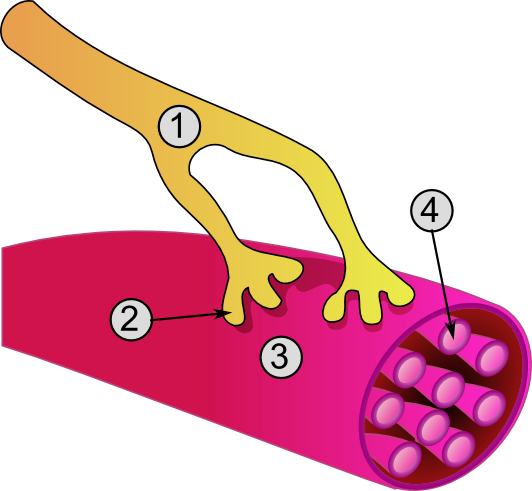
\includegraphics[height=5cm]{munit}}
\end{center}
\end{figure}
In this study, data are collected using two MYO armbands \cite{myo}, on the upper arm of the subject (just above the elbow), as seen in \autoref{fig:myoplace}. Intuitively, the idea is to collect the signal where the sensors are, and classify them with enough speed that it feels as if the hand were being moved on its own.
\begin{figure}[h]
\caption{%
The MYO armbands are placed just above the elbow.
}
\label{fig:myoplace}
\begin{center}
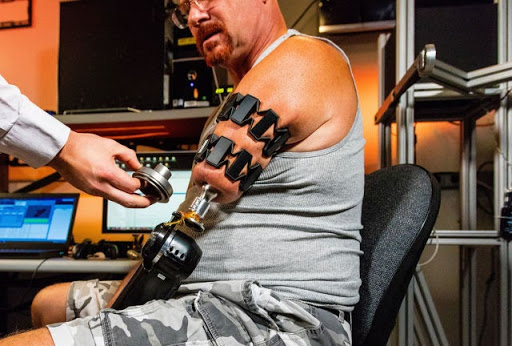
\includegraphics[scale=0.5]{myoplace}
\end{center}
\end{figure}


\subsection{The NinaPro Database}

The data in this study comes from the NinaPro Database, specifically database number 5 \cite{nina5}. Within this database, there are 52 unique motions measured, as well as rest, collected over 10 subjects. Each subject does each exercise 6 times, with 3 seconds of rest between each repetition. The signal from these are collected at the frequency of the MYO armband, 200 Hertz. 
\par This is one of the big challenges and benefits of the MYO armband. Low frequency sEMG is very sparse in information, and thus difficult to classify (especially relative to expensive HDsEMG sensors), however this also means that the MYO armband is cheap and accessible to the average consumer. The other benefit of MYOs cheapness and sparsity can be inferred from \autoref{fig:myoplace}. The cheap sensor constricts the arm and stays in place. Because the signals are weaker, slight shifts in the electrode do not have as much of an impact on the underlying signal (as the sensor is not incredibly sensitive). This means that the MYO armband is simpler and more robust for use by the general public.\par

The goal of this study is to develop an accurate mapping between MUAP in the upper arm and the motion of the hands.

